\section{Quasimodularity of the generating function}

In this section, we use a formula of Frobenius to express the function $\widehat{Z}(q,\lam)$ as the constant term of a certain product of Laurent series. This is exactly what is needed to prove that the generating function $F_g$ is quasimodular for $g\geq 2$, using the theorem about the generalized Jacobi function found in \cite{Kaneko-Zagier1995}. The formula also exhibits a way to concretely compute the number of disconnected covers of given genus and degree.

\subsection{Subsets of the half integers}

Recall that the irreducible characters of $\Sym_d$ are parametrized by Young diagrams of size $d$. %TODO maybe example?
We will make use of the set of \emph{positive half integers} $\pai$.

\begin{prop} \label{prop:bijection-young}
 There is a bijection between the set of Young diagrams of size $d$ and the set of pairs $(U,V)$ of finite subsets of $\pai$ such that $\abs{U}=\abs{V}$ and $d=\sum_{u\in U}u + \sum_{v\in V}v$.
\end{prop}
\begin{center}
 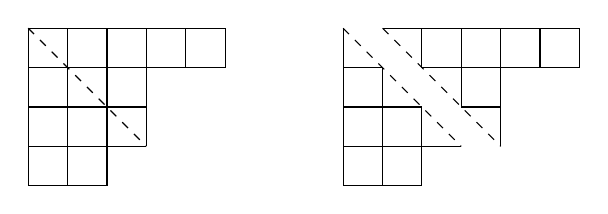
\begin{tikzpicture}[scale=0.50]
  \draw (0,0) -- (0,4);
  \draw (1,0) -- (1,4);
  \draw (2,0) -- (2,4);
  \draw (3,1) -- (3,4);
  \draw (4,3) -- (4,4);
  \draw (5,3) -- (5,4);
  
  \draw (0,0) -- (2,0);
  \draw (0,1) -- (3,1);
  \draw (0,2) -- (3,2);
  \draw (0,3) -- (5,3);
  \draw (0,4) -- (5,4);
  
  \draw[dashed] (0,4) -- (3,1);
  
  \draw (8,0) -- (8,4);
  \draw (9,0) -- (9,3);
  \draw (10,0) -- (10,2);
  
  \draw (8,3) -- (9,3);
  \draw (8,2) -- (10,2);
  \draw (8,1) -- (11,1);
  \draw (8,0) -- (10,0);
  
  \draw[dashed] (8,4) -- (11,1);
  
  \draw (10,3) -- (10,4);
  \draw (11,2) -- (11,4);
  \draw (12,1) -- (12,4);
  \draw (13,3) -- (13,4);
  \draw (14,3) -- (14,4);
  
  \draw (9,4) -- (14,4);
  \draw (10,3) -- (14,3);
  \draw (11,2) -- (12,2);
  
  \draw[dashed] (9,4) -- (12,1);

 \end{tikzpicture}
\end{center}

\begin{proof}
 Consider any a Young diagram of size $d$. Starting with the upper left corner, cut it diagonally in two pieces (see picture). This gives $s$ ``cut'' columns in the lower piece and $s$ ``cut'' rows in the upper piece. Let $u_i\in\pai$ denote the number of squares in the $i$-th cut row and $v_i$ the number of squares in the $i$-th cut column. Define $U=\{u_1,\dotsc,u_s\}$ and $V=\{v_1,\dotsc,v_s\}$. Then $|U|=|V|$ and $d=\sum_{u\in U}u + \sum_{v\in V}v$. Conversely, let two such $U$ and $V$ be given. The associated Young diagram is obtained by arranging both $U$ and $V$ in ascending order and then iteratively gluing the rows with $u_i$ squares to the columns with $v_i$ squares, for the appropriate elements $u_i \in U$ and $v_i \in V$ respectively.
\end{proof}

\begin{prop} \label{prop:frobenius-formula}
 Let $\chi$ be the character associated to the Young diagram corresponding to the subsets $U,V\in\pai$ of equal cardinality $s$. Then
 \[
  \frac{\binom{d}{2} \chi(t)}{\dim(\chi)} = \frac{1}{2}\left(\sum_{i=1}^s u_i^2 - \sum_{i=1}^s v_i^2\right).
 \]
\end{prop}
\begin{proof}
 See \cite{Fulton-Harris91}, p. 52.
\end{proof}

\begin{defi}
 Define the Laurent series $\theta(\zeta,q,\lam)$ in $\zeta$ with coefficients formal power series in $q$ and $\lam$ as follows:
 \[
  \theta(\zeta,q,\lam) = \prod_{u\in\pai} \left(1+\zeta q^u e^{u^2\lam/2}\right) \prod_{v\in\pai} \left(1+\zeta^{-1} q^v e^{-v^2\lam/2}\right).
 \]
\end{defi}

\begin{lemma} \label{prop:theta-expansion}
 The counting function $\what{Z}(q,\lam)$ is the coefficient of $\zeta^0$ in the series $\theta(\zeta,q,\lam)-1$.
\end{lemma}
\begin{proof}
 By expanding the product, one finds that $\theta(\zeta,q,\lam)=\sum_{U,V\subset\pai}a_{U,V}$, where \[a_{U,V}=\zeta^k q^d \exp(\mu_{U,V}\lam).\] Here, \begin{enumerate} \item $k=\abs{U}-\abs{V}$
 \item $d=\sum_{u\in U}u + \sum_{v\in V}v$
 \item $\mu_{U,V}=\frac{1}{2}\left(\sum_{i=1}^s u_i^2 - \sum_{i=1}^s v_i^2\right)$.
 \end{enumerate}
Using the bijection in proposition \ref{prop:bijection-young}, let the eigenvalues of the matrix $M_d$ be indexed by pairs $(U,V)$ of subsets of $\pai$ such that $\abs{U}=\abs{V}$ and $d=\sum_{u\in U}u + \sum_{v\in V}v$. By lemma \ref{prop:eigenvalues} and proposition \ref{prop:frobenius-formula}, the eigenvalue indexed by the pair $(U,V)$ is equal to $\mu_{U,V}$.

Now consider the coefficient of $\zeta^0$ in $\theta(\zeta,q,\lam)-1$. There, the coefficient of $q^d$ is $\sum_{U,V}\exp({\mu_{U,V}\lam})$, where the $\mu_{U,V}$ are the eigenvalues of $M_d$. By \ref{prop:counting-fct}, this sum is equal to the coefficient of $q^d$ in $\what{Z}(q,\lam)$. This proves the lemma.
\end{proof}

\subsection{The coefficients of the theta function}

Recall that $F_g$ was defined as the series

 \[Z(q,\lam) = \sum_{g\geq 1}\frac{F_g(q)}{(2g-2)!}\lam^{2g-2}.\]
 
For an element $\tau$ of the upper half plane, set $q=\exp(2\pi i \tau)$ Sometimes $q$ will be viewed as a formal variable.

\begin{prop} \label{prop:exp-quasimodular}
 Let $a(x)=\sum_{k\geq 1} a_k x^k$ be a formal power series in $x$, with holomorphic functions $a_k$ on the upper half plane as coefficients. Let $\exp(a(x))=\sum_{k\geq 1} b_k x^k$ be its formal exponential. Assume that each of the coefficients $b_k$ is quasimodular of weight $kr$, for some $r$. Then the $a_k$ are also quasimodular of weight $kr$.
\end{prop}
\begin{proof}
 This follows essentially by computing by hand the coefficients $b_i$.
\end{proof}

\begin{defi}
 Define the Laurent series $\Theta(\zeta,q,\lam)$ in $\zeta$ with formal power series in $q$ and $\lam$ as coefficients by
 \[
  \Theta(\zeta,q,\lam)=(\prod_{n\geq 1}(1-q^n))\theta(\zeta,q,\lam).
 \]
 Further, let $\Theta_0(q,\lam)$ denote the coefficient of $\zeta^0$ in $\Theta(\zeta,q,\lam)$.
\end{defi}

The following theorem about the quasimodularity of the coefficients of $\Theta_0$ is proved in \cite{Kaneko-Zagier1995}.

\begin{thm}
 Let $\Theta_0(q,\lam)=\sum_{k}A_k(q)\lam^k$ be the constant $\zeta$-coefficient of $\Theta$. Then the coefficient $A_k(q)$ is a quasimodular form of weight $3k$.
\end{thm}

We may now prove the main result:

\begin{thm}[\cite{Dijkgraaf}]
 For $g\geq 2$, the function $F_g(q)$ is a quasimodular form of weight $6g-6$.
\end{thm}
\begin{proof}
 Lemma \ref{prop:theta-expansion} gives the equality
 \begin{equation} \label{eq:theta-expansion}
  \Theta_0(q,\lam)=(\prod_{n\geq 1}(1-q^n))(\what{Z}(q,\lam)+1).
 \end{equation}
 By the previous theorem, the coefficient of $\lambda^{2g-2}$ in this product is quasimodular of weight $6g-6$. By Lemma \ref{prop:connection-reduction} one obtains, after taking the logarithm of both sides of \eqref{eq:theta-expansion},
 \[
  \log\Theta_0(q,\lam)=\sum_{n\geq 1}\log(1-q^n) + Z(q,\lam).
 \]
 As seen in Example \ref{ex:genus-one}, we have $F_1=-\sum_{n\geq 1}\log(1-q^n)$. Hence, in $\log\Theta_0(q,\lam)$ the coefficient of $\lambda^0$ is zero. Thus, we may apply proposition \ref{prop:exp-quasimodular} and the previous theorem to find that the coefficient of $\lambda^{2g-2}$ in $\log\Theta_0(q,\lam)$, that is $F_g(q)/(2g-2)!$, is a quasimodular form of weight $6g-6$. This concludes the proof.
\end{proof}


